% --------------------------------------
% Chapter 13 Solutions
% --------------------------------------


\subsection{13.1 $\bigstar\bigstar\bigstar$}

We are given that 
\begin{itemize}
\item[$\clubsuit$] $1\cdot a=a$
\item[$\bigstar$] $a^{-1}a=1$
\item[$\blacksquare$] $a(bc)=(ab)c$
\end{itemize}
where $a,b,c\in G$, where $G$ is some set. First we want to show that $a\cdot 1=a$. So
\begin{align*}
a^{-1}(a \cdot 1)=(a^{-1}a)\cdot 1=1\cdot 1=1
\end{align*}
Now we prove that inverses are unique. Suppose there exists $b\neq a$, such that $a^{-1}b=1$. Then letting $d=a^{-1}$, we have that
\begin{align*}
a^{-1}b&=db=1\\
\implies \ \ \ \ (d^{-1}d)b&=d^{-1}\cdot 1\\
\implies \ \ \ \ \ \ \ \ \  1\cdot b&=d^{-1}\cdot 1\\
\implies \ \ \ \ \ \ \ \ \ \ \  bd&=d^{-1}\cdot 1\cdot d\\
\implies \ \ \ \ \ \ \ \ \ \ \ bd&=1\\
\implies \ \ \ \ \ \ ba^{-1}a&=1\cdot a\\
\implies \ \ \ \ \ \, \ \ \ \ \ \ \  b&=a\\
\end{align*} 
Contradiction! Hence our assumption that $b\neq a$ is false, and so $b=a$. In our case, we have that $b=a\cdot 1=a$, as we wanted to show.\\ \\
We now want to show that $aa^{-1}=1$. 
$$(aa^{-1})a=a(a^{-1})a)=a\cdot 1 = a$$
If we can show that the identity is unique, then we will have our result. So suppose there is $c\neq 1$ and that $ca=a$ \emph{for all $a\in G$}. Hence
\begin{align*}
ca^{-1}&=a^{-1}\\
\implies \ \ \ \ c(a^{-1}a)&=a^{-1}a\\
\implies \ \ \ \ \ \ \ \ \ c\cdot 1&=1\\
\implies \ \ \ \ \ \ \ \ \ \ \, \ \ c&=1\\
\end{align*}
The first line holds as $a^{-1}\in G$ and hence $c a^{-1}=a^{-1}$ by assumption. Thus we have a contradiction, and our assumption that $c\neq 1$ is false, and hence $c=1$. In our case, we have that $c=aa^{-1}=1$, as we wanted. \\ \\
The next part we will approach by providing a set whose elements obey $\bigstar$, $\blacksquare$ and $a1=a$, but not $1a=a$ and $aa^{-1}=1$.\\ So let us have a set $G=\{1,a\}$. It has the multiplication rules $a1=a$, $1 a=1$, $11=1$ and $aa=a$. This set certainly obeys $a1=a$, and also $\bigstar$ with $a^{-1}=1$ and $1^{-1}=1$. Then to check $\blacksquare$, there are 8 combinations to check. These are easy to do. Here are two:
\begin{align*}
&a(a1)=aa=a=(aa)1\\
&1(1a)=11=1=(11)a
\end{align*}
Checking the rest, we see that $\blacksquare$ is satisfied. But $1a=1\neq a$ and $aa^{-1}=a1=a\neq 1$. Hence $a1=a$, $\blacksquare$ and $\bigstar$ cannot imply $\clubsuit$ and $aa^{-1}=1$.


\subsection{13.4 $\bigstar \bigstar $}
We are asked to show that the multiplication table of the group $\{1,-1,i,-i,\mathbf{C},\mathbf{C}i,-\mathbf{C},-\mathbf{C}i\}$ can deduced from three identities
\begin{equation}\label{134}i^4=1, \ \ \ \mathbf{C}^2=1 \ \ \ \ \mathbf{C}i=i^3\mathbf{C}\end{equation}
 Now there is some confusion as to what Penrose wanted us to assume. If all we know about the group are the above three properties, we can't deduce all the rules (For example, how does one deduce that 1.1=1 for example, or that $i^2=-1$?). It seems we are expected to interpret the group elements $1,-1,i,-i$ as normal complex numbers, for which we know the multiplication rules. (But then we know what $i^4$ is, and so Penrose could have given only two rules to work out the multiplication table...)\\ \\ With this in mind, we see that we can deduce the group multiplication laws from the multiplication laws shown in Question [13.3] Now we show that these follow from \eqref{134}. The first:
$$
\mathbf{C}i=i^3\mathbf{C}\implies i\mathbf{C}i=(i^4)\mathbf{C}\implies (i^2)\mathbf{C} i =i\mathbf{C}\implies -\mathbf{C} i = i\mathbf{C}\implies \mathbf{C}i=(-i)\mathbf{C}$$
The second:
$$\mathbf{C}i=(-i)\mathbf{C}\implies i = \mathbf{C}(-i)\mathbf{C}\implies i^2=\mathbf{C}(-i)\mathbf{C}i\implies \mathbf{C}(-1)=\mathbf{C}(-i)\implies\mathbf{C}i=(-i)i^3\mathbf{C} $$


\subsection{13.6 $\bigstar \bigstar $}
We enumerate the various possible subgroups of $G=\{1,-1,i,-i,\mathbf{C},\mathbf{C}i,-\mathbf{C},-\mathbf{C}i\}$, and see which of these are non-normal. 
\begin{itemize}
\item 1 must be in any subgroup
\item {1,-1} is subgroup, but normal as 1,-1 commute with all elements of $G$.
\item The smallest subgroup containing $i$ or $-i$ is $\{1,i,-i,-1\}$. This subgroup is normal. This follows from $$\mathbf{C}\{1,i,-i,-1\}=\{\mathbf{C},\mathbf{C}i,\mathbf{C}(-i),\mathbf{C}(-1)\}=\{\mathbf{C},(-i)\mathbf{C},i\mathbf{C},(-1)\mathbf{C}\}=\{1,i,-i,-1\}\mathbf{C}$$
This shows that any rotation followed by a reflection can also me made of a reflection first and then a rotation. We don't have to check the other reflections, as they are simply rotations composed with a reflection. 
\item Reflecting twice about the same axes always give us back the identity, so each reflection with the identity is a subgroup. These are $\{1, \mathbf{C}\}$,$\{1, \mathbf{C}i\}$, $\{1, -\mathbf{C}\}$ and $\{1, -\mathbf{C}i\}$. These are each non-normal, which can be seen by post- and pre-multiplying the group by $i$, as Penrose did.
\item Expanding these groups by adding $i$ or $-i$ gives us the trivial normal group.
\item Expanding by adding -1 gives us two groups of order 4, $\{1,-1, \mathbf{C},-\mathbf{C}\}$ and $\{1,-1, \mathbf{C}i,-\mathbf{C}i\}$. But these subgroups are normal. Multiplying any of the elements by $i$ would lead to at most a difference of $-1$ between pre- and post-multiplying. Also, $(\mathbf{C}i)C=(i^3\mathbf{C})\mathbf{C}=-i$ and $\mathbf{C}(\mathbf{C}i)=i$. Again differing only by $-1$, and hence the two subgroups are normal.  
\end{itemize}
The above are the only possible subgroups, and hence there are only 4 non-normal subgroups.


\subsection{13.7 $\bigstar \bigstar\bigstar $}
We are asked to show that $SO(3)$ is the only non-trivial normal subgroup of $O(3)$. First we show that $SO(3)$ is a normal subgroup. Here are some facts we will need, all follow from something stated or proven in Chapter 13.
\begin{itemize}
\item Let $\mathbf{O}$ be a $3\times 3$ matrix. Then $\mathbf{O}\in O(3)$ iff $\mathbf{O}\mathbf{O}^T=\mathbf{I}$.
\item   Let $\mathbf{A}$ be a $3\times 3$ matrix. Then $\mathbf{A}\in SO(3)$ iff $\mathbf{A}\in O(3)$ and $\det\mathbf{A}=1$.
\item $\det( \mathbf{AB})=\det(\mathbf{A})\det(\mathbf{B})$
\item $\det(\mathbf{A}^T)=\det(\mathbf{A})$
\item $H$ is a normal subgroup of $G$ iff $g H=Hg$ where $g\in G$ $\iff$ $H=gH g^{-1}\iff gh g^{-1}\in H $ for all $h\in H$.
\end{itemize} 
Its easy to see that $SO(3)$ is a subgroup. It is closed (if $\mathbf{A},\mathbf{B}\in SO(3)$, then $\det(\mathbf{A}\mathbf{B})=\det(\mathbf{A})\det(\mathbf{B})=1\cdot 1=1$, so $\mathbf{A}\mathbf{B}\in SO(3)$), it contains the identity \textbf{I}, and inverses (if $\det(\mathbf{A})=1$, then $\det(\mathbf{A}^T)=1$. And so if $\mathbf{A}\in SO(3)$, then its inverse $A^{-1}=A^T\in SO(3)$). \\ \\ It is also easy to see that it is a normal subgroup, as iff $\mathbf{A}\in SO(3)$, and $\mathbf{X}\in O(3)$, then $\det(\mathbf{X}\mathbf{A}\mathbf{X}^{-1})=\det(\mathbf{X})\det(\mathbf{A})\det(\mathbf{X}^T)=[\pm 1]^2 \cdot 1=1$, and so $\mathbf{X}\mathbf{A}\mathbf{X}^{-1}\in SO(3)$ which means $SO(3)$ is normal.  \\ \\ Now we need to show that there are no other normal subgroups of $O(3)$. We will examine two cases:
\begin{itemize}
\item[1.] Can we create any normal subgroups if we include reflections?
\item[2.] Are there any normal subgroups of $SO(3)$?
\end{itemize}
\subsubsection*{Case 1 - Including reflections}
Let $\mathbf{T}$ be some reflection. Now the simplest group containing a least 1 reflection is $\mathcal{G}=\{\mathbf{I},\mathbf{T}\}$, where $\mathbf{I}$ is the identity. Its a group, as for any reflection $\mathbf{T}^2=\mathbf{I}$. But this is certainly not a normal subgroup. Look at Figure 1. We choose our coordinate system so that $\mathbf{T}$ is a reflection about the $xz-$plane. The action of $\mathbf{T}$ on the point $(-1,0)$. It leaves it invariant. Let $\mathcal{R}_\theta\in O(3)$ be an anticlockwise rotation of $\theta$ about the origin. If $\mathcal{G}$ were a normal subgroup, then $\mathcal{R}_{-\theta}\circ\mathbf{T}\circ \mathcal{R}_{-\theta}\in \mathcal{G}$, which it obviously is not from Figure 1. The element $\mathcal{R}_{-\theta}\circ\mathbf{T}\circ \mathcal{R}_{-\theta}$ is a reflection about the blue line. \\ But what if we try and enlarge $\mathcal{G}$ so that it is normal? To do this, we immediately have to add the reflection planes intersecting the blue lines. But $\theta$ was arbitrary, and so every reflection plane through each opposite points on the circle will have to be added.\\ \\ But this is not yet big enough, as we can use the same argument with a reflection plane about the $yz-$plane and the $xy-$plane. We must conclude that our group must include all reflections to stand a chance of being normal. But now we use a key fact: Any rotation is the composition of two reflections. So for a group containing all reflections to be closed, we need to include all the rotations. But this is just a trivial subgroup of $O(3)$, namely $O(3)$ itself.  
\begin{figure}
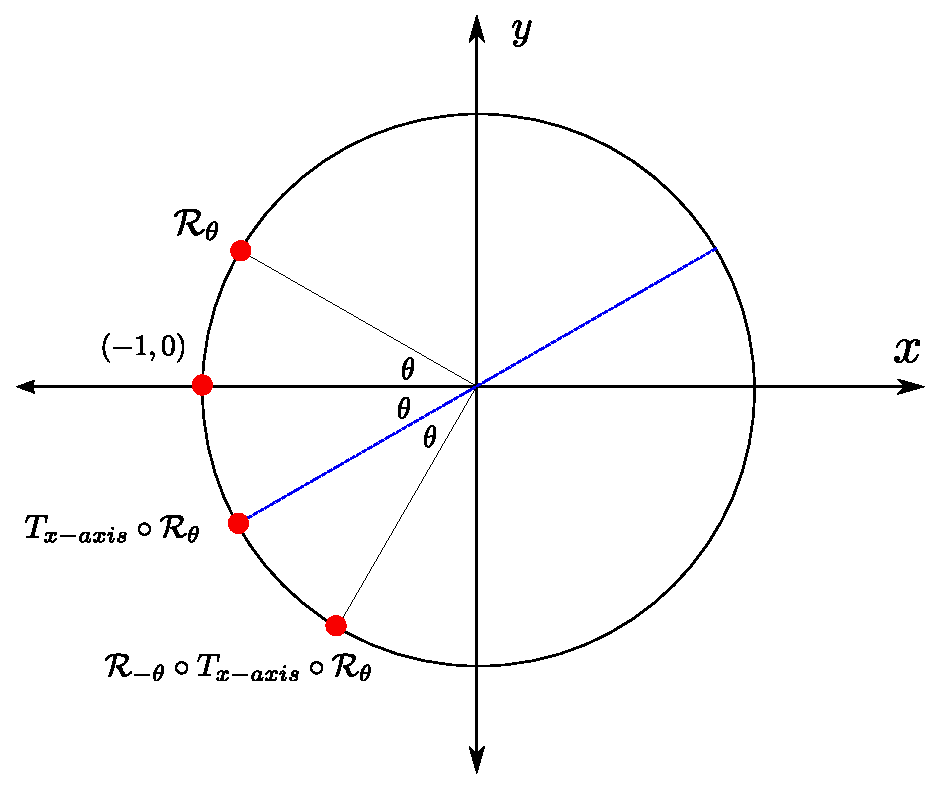
\includegraphics[scale=0.6]{chapters/images/13.7.eps}
\caption{}
\end{figure} 
\subsubsection*{Case 2 - Only rotations}
We will now show that there are no subgroups of $SO(3)$ which can be normal with respect to $O(3)$. We could do this using a similar technique to Case 1, but it is a little messy. A more elegant method is to use quaternions. \\ \\ We will need some facts which Penrose doesn't explicitly state, but could be derived if clever enough.
\begin{itemize}
\item The quaternion $\mathbb{V}=\cos \frac{\theta}{2}+\sin \frac{\theta}{2}(v_1\textbf{i}+v_{2}\textbf{j}+v_{3}\textbf{k})=\cos \frac{\theta}{2}+\sin \frac{\theta}{2}\mathbf{V}$ where $\mathbf{V}$ is a unit vector, represents a rotation of $\theta$ about the axis $\mathbf{V}$.
\item Suppose we have some 3-d vector $\mathbf{W}$. Then $\mathbf{W}'=\mathbb{V}\mathbf{W}\mathbb{V}^{-1}$ is $\mathbf{W}$ rotated about $\mathbf{V}$ by an angle $\theta$.
\end{itemize}
Now suppose there exists a non-trivial normal subgroup of $SO(3)$. Then it must contain some rotation represented by a quaternion of the form $\mathbb{W}=\cos \frac{\phi}{2}+\sin \frac{\phi}{2}(w_1\textbf{i}+w_{2}\textbf{j}+w_{3}\textbf{k})=\cos \frac{\phi}{2}+\sin \frac{\phi}{2}\mathbf{W}$. Obviously $\phi\neq 2\pi$, and let us assume also for now that $\phi\neq \pi$. Now for the subgroup containing $\mathbb{W}$ to be normal, it must also contain all elements of the form \begin{align*}
\mathbb{V}\mathbb{W}\mathbb{V}^{-1}=\mathbb{V}(\cos \frac{\phi}{2}+\sin \frac{\phi}{2}\mathbf{W})\mathbb{V}^{-1}=\cos \frac{\phi}{2}\cdot 1+\sin \frac{\phi}{2}\mathbb{V}\mathbf{W}\mathbb{V}^{-1}
\end{align*}
As $\mathbb{V}$ is arbitrary, $\mathbb{V}\mathbf{W}\mathbb{V}^{-1}$ is an arbitrary rotation of the unit vector $\mathbf{W}$, and so $\mathbb{V}\mathbf{W}\mathbb{V}^{-1}$ is also an arbitrary vector. Hence the subgroup containing the rotation $\mathbb{W}$ must also contain rotations of $\phi$ about \emph{every rotation axis}. \\ \\ Now we demand that this group be closed, and show that this further requirement generates the whole of $SO(3)$.  \\ \\ We know that our potential normal subgroup contains a rotation of $\phi$ about the $z-$axis. Now we need to show that for any $\theta$, a rotation of $\theta$ about the $z-$axis must also be in our subgroup. This is easy. Suppose we have a point $\mathbf{A}=(0,\frac{\pi}{2})$ and a point $\mathbf{B}=(\theta,\frac{\pi}{2})$.  


\subsection{13.9 $\bigstar \bigstar $}
Let us denote the order of the group $\mathcal{G}$ by $|\mathcal{G}|$. We are trying to show that $|\mathcal{G}/\mathcal{S}|=|\mathcal{G}|/|\mathcal{S}|$. Now let $H$ be the set $H=\mathcal{G}-\mathcal{S}$, ie. all the elements of $\mathcal{G}$ not in $\mathcal{S}$. We will need the following simple results:
\begin{itemize}
\item[1.] If $s\in\mathcal{S}$, then $s*\mathcal{S}=\mathcal{S}$, the identity element.
\item[2.] The order of $H$ is $|H|=|\mathcal{G}|-|\mathcal{S}|$.
\item Suppose $h_1\in H$ and $s\in\mathcal{S}$. Then $h_1* s\in H$. This is easy to show, as suppose that $h_1*s\in \mathcal{S}$. Then $h_1 *s*s^{-1}=h_1\in \mathcal{S}$, which is a contradiction.
\item[3.] Let $h_1\in H$. Then $h_1$ maps each element of $\mathcal{S}$ into a unique element of $H$. Uniqueness is easy to show, as $h_1*s_1=h_1*s_2\implies s_1=s_2$
\item[4.] Let $H_1=h_1*\mathcal{S}$. Then $|H_1|=|\mathcal{S}|$. This follows from the last two points.
\item[5.] Let $H_1=h_1*\mathcal{S}$. Now suppose $h_2\notin H_1$. Then $h_2*s \notin H_1$. To see this, suppose there is some $s_1,s_2\in \mathcal{S}$, such that $h_1*s_1=h_2*s_2$. Then $h_2=h_1*s_1*s^{-1}_{2}$. But there is some $s\in \mathcal{S}$ such that $s=s_1*s^{-1}_{2}$. Then $h_2=h_1*s\in H_1$. Contradiction!
\end{itemize}
We can thus conclude that after applying each of the elements of $H$ to $\mathcal{S}$, we get a collection of sets $H_1,H_2,\ldots H_n$. These sets are non-intersecting (from point 5.) and each of order $|\mathcal{S}|$ (point 4.). Thus the number $n$ of of these sets must be 
$$n=\frac{|H|}{|\mathcal{S}|}=\frac{|\mathcal{G}|-|\mathcal{S}|}{|\mathcal{S}|}=\frac{|\mathcal{G}|}{|\mathcal{S}|}-1$$
Each of these sets is an element of $\mathcal{G}/\mathcal{S}$ But we haven't counted in $\mathcal{S}$, which is the identity element. Including this, we get
$$|\mathcal{G}/\mathcal{S}|=\frac{|\mathcal{G}|}{|\mathcal{S}|}-1+1=\frac{|\mathcal{G}|}{|\mathcal{S}|}$$
From another perspective, we have shown that the sets $g*\mathcal{S}$, where $g\in \mathcal{G}$, form a partition of $\mathcal{G}$, meaning that either $(g_1*\mathcal{S})\cap (g_2*\mathcal{S})=\emptyset$ or $(g_1*\mathcal{S})= (g_2*\mathcal{S})$, and that the union of all these sets is just the set $\mathcal{G}$. Knowing this, and that each set $g\in \mathcal{G}$ has order $\mathcal{S}$, the result follows easily.   \\ \\ \textbf{Note:} Sharp-eyed readers might wonder what would happen if $|\mathcal{S}|$ does not divide $|\mathcal{G}|$. Surely a group can't have a fractional order! Indeed not. The resolution to the problem is that the order of any subgroup of a group $\mathcal{G}$, must divide the order of the group $\mathcal{G}$. This is known as \emph{Lagrange's Theorem}, which we have effectively proven. A simple consequence, for example, is that a group of prime order cannot have any (non-trivial) subgroups. pp


\subsection{13.17 $\bigstar \bigstar $}
Suppose there exists $\mathbf{v}_1\neq \mathbf{0}$ such that $\mathbf{T}\mathbf{v}_1=\mathbf{0}$. Now suppose our vector space $\mathbb{V}$ is of dimension $n$. Then we can always find a set of $n$ linearly independent vectors $\{\mathbf{v}_1,\mathbf{v}_2,\ldots,\mathbf{v}_n\}$ such that an arbitrary vector $\mathbf{w}\in\mathbb{V}$ can be written as a linear combination of these vectors.\\ Now let $\mathbb{W}_{\mathbf{T}}=\{\mathbf{T}\mathbf{u}:\mathbf{u}\in \mathbb{V}\}$. An arbitrary element of $\mathbb{W}_{\mathbf{T}}$ can be written
\begin{align*}
\mathbf{T}\mathbf{w}&=\mathbf{T}(\alpha_1 \mathbf{v}_1+\alpha_2 \mathbf{v}_2+\ldots \alpha_n \mathbf{v}_n)\\
&=\alpha_1 \mathbf{T}\mathbf{v}_1+\alpha_2 \mathbf{T}\mathbf{v}_2+\ldots \alpha_n \mathbf{T}\mathbf{v}_n\\
&=\mathbf{0}+\alpha_2 \mathbf{T}\mathbf{v}_2+\ldots \alpha_n \mathbf{T}\mathbf{v}_n\\
\end{align*} 
And so the set $\{\mathbf{T}\mathbf{v}_2,\mathbf{T}\mathbf{v}_3,\ldots  ,\mathbf{T}\mathbf{v}_n\}$ forms a basis for $\mathbb{W}_{\mathbf{T}}$. But it has only $n-1$ elements, and so its dimension is smaller than that of $\mathbb{V}$, and hence is singular.\\ \\ I think Penrose made a mistake with his hint, as he no where mentions the determinant condition, which is that $\mathbf{T}$ is singular iff $\det \mathbf{T}=0$. Then a simple fact about determinants is that iff you swop two rows or columns, then the determinant picks up a minus sign. But if there are two rows which are the same, then swopping them leaves $\mathbf{T}$ unchanged, and so $\det \mathbf{T}=-\det\mathbf{T}\implies \det \mathbf{T}=0$. It is also obvious that if there is a row or column of zeroes, then the determinant is also zero.


\subsection{13.18 $\bigstar \bigstar $}
I am not completely sure what Penrose means by `not using explicit expressions'. \\ \\ The key fact we will use is that any bijective map has an inverse. (This should be intuitively obvious.) We assume that $\mathbf{T}$ is non-singular. In our case, we obviously don't have to worry about $\mathbf{T}$ being surjective (onto). So let us show it is injective (one-to-one). Now suppose $\mathbf{T}\mathbf{v}=\mathbf{T}\mathbf{u}\implies \mathbf{T}(\mathbf{v}-\mathbf{u})=\mathbf{0}
$. But $\mathbf{T}$ is non-singular, and so $\mathbf{v}-\mathbf{u}=\mathbf{0}\implies \mathbf{v}=\mathbf{u}$ and so $\mathbf{T}$ is injective, and hence bijective, and hence has an inverse.\\ \\ Another way of seeing this is to note that two vector spaces $\mathbb{V}$ and $\mathbb{W}$ of the same dimension are basically the same, as they have an equivalent number of basis vectors. One can easily find a linear map mapping the basis vectors of $\mathbb{W}$ to basis vectors of $\mathbb{V}$. Then the inverse of this map simply maps the basis vectors of $\mathbb{V}$ to those of $\mathbb{W}$.


\subsection{13.25 $\bigstar\bigstar\bigstar$}
We present three proofs here. The first is what I think Penrose wanted, and relies on the Jordan Canonical form, which is reffered to in Footnote \textbf{12} (whilst the second and third do not). The second is what I consider the most elegant, whilst the third I found somewhere and relies on the least amount of matrix algebra facts.\\ \\ For the first and second proof, we need the fact that for any $n\times n$ matrix $\mathbf{A}$, which has eigenvalues $\lambda_1,\lambda_2,\ldots,\lambda_n$, 
\begin{align*}
\det \mathbf{A}&=\lambda_1\lambda_2\ldots\lambda_n\\
\text{trace}\mathbf{A}&=\lambda_1+\lambda_2+\ldots+\lambda_n
\end{align*} 
which we found in Question \textbf{[13.27]}.
\subsubsection*{Proof 1}
Following Penrose, we first assume the eigenvalues of \textbf{A}, $\lambda_1,\lambda_2,\ldots,\lambda_n$ are distinct, and show that 
$$\det e^\textbf{A}=e^{\text{trace}\,\textbf{A}}$$ 
holds for this case. We immediately have, iff \textbf{A} is an $n\times n$ matrix, that
$$e^{\text{trace}\,\textbf{A}}=e^{\lambda_1+\lambda_2+\ldots+\lambda_n}$$
As the eigenvalues are distinct, we can always choose the eigenvectors of \textbf{A} as the basis, and so express \textbf{A} in the Canonical form. In this basis, it can easily be seen that
$$\textbf{A}^k=
\begin{pmatrix} 
\lambda_{1}^{k}&0 &\ldots&0\\
0&\lambda_{2}^{k}&\ldots&0\\
\vdots & \vdots & \ldots &\vdots \\
0&0&\ldots &\lambda_{n}^{k}
\end{pmatrix}$$
Hence
\begin{align*}
\det e^\textbf{A}&=\det \left ( 1+\textbf{A}+\frac{\textbf{A}^2}{2!}+\ldots\right)\\
&=\det \begin{pmatrix} 
1+\lambda_{1}+\frac{\lambda_{1}^{2}}{2!}+\ldots&0 &\ldots&0\\
0&1+\lambda_{2}+\frac{\lambda_{2}^{2}}{2!}+\ldots&\ldots&0\\
\vdots & \vdots & \ldots &\vdots \\
0&0&\ldots &1+\lambda_{n}+\frac{\lambda_{n}^{2}}{2!}+\ldots
\end{pmatrix}\\
&=\det \begin{pmatrix} 
e^\lambda_1&0 &\ldots&0\\
0&e^\lambda_2&\ldots&0\\
\vdots & \vdots & \ldots &\vdots \\
0&0&\ldots &e^\lambda_n
\end{pmatrix}\\
&=e^{\lambda_1+\lambda_2+\ldots+\lambda_n}=e^{\text{trace}\,\textbf{A}}
\end{align*}
Now when the eigenvalues are degenerate, the we cannot necessarily express \textbf{A} in the Canonical form. But according to Footnote \textbf{12}, we can find a basis for \textbf{A} such that it will be in the Canonical form with at most some ones in the next diagonal.\\ This Jordan Canonical form is evidently an upper triangular matrix. Two easy to see facts about upper triangular matrices are that iff \textbf{A} is upper triangular, then $\det (\textbf{A})=a_{11}a_{22}\ldots a_{nn}$, and the product of two upper triangular matrices is also upper triangular. The last thing we note is that iff \textbf{A} and \textbf{B} are upper triangular, and \textbf{A}\textbf{B}=\textbf{C}, then $c_{ii}=a_i\, b_i$. Using these facts, it is easy to see that the proof for Canonical matrices will extend exactly to matrices in the Jordan canonical form, and so degeneracies in the eigenvalues can't falsify the expression $\det e^\textbf{A}=e^{\text{trace}\,\textbf{A}}$.\\ \\ 

\subsubsection*{Proof 2}
The method of this proof is to find the eigenvalues of $e^{\mathbf{A}}$, and then find $\text{det}\,e^\mathbf{A}$. Now suppose \textbf{A} is again an $n\times n$ matrix with eigenvalues $\lambda=\lambda_1,\lambda_2,\ldots,\lambda_n$. Also, \textbf{v} is an $n\times 1$ column vector. Then we immediately have that $\mathbf{A}^n\mathbf{v}=\lambda^n\mathbf{v}$, and so
\begin{align*}
e^\mathbf{A}\mathbf{v}&=\left (\mathbf{I}+\frac{\mathbf{A}}{1!}+\frac{\mathbf{A}^2}{2!}+\frac{\mathbf{A}^3}{3!}+\ldots\right )\mathbf{v}\\
&=\left (\mathbf{I}\mathbf{v}+\frac{\mathbf{A}\mathbf{v}}{1!}+\frac{\mathbf{A}^2\mathbf{v}}{2!}+\frac{\mathbf{A}^3\mathbf{v}}{3!}+\ldots\right )\\
&=\left (1\cdot\mathbf{v}+\frac{\lambda\cdot\mathbf{v}}{1!}+\frac{\lambda^2\cdot\mathbf{v}}{2!}+\frac{\lambda^3\cdot\mathbf{v}}{3!}+\ldots\right )\\
&=e^\lambda \cdot \mathbf{v}\\
\end{align*}
So iff $\lambda$ is an eigenvalue of \textbf{A}, then $e^\lambda$ is an eigenvalue of $e^\mathbf{A}$. Hence 
\begin{align*}
\text{det}\,e^\mathbf{A}&=e^{\lambda_1}\cdot e^{\lambda_2}\cdot \ldots \cdot e^{\lambda_n}\\
&=e^{\lambda_1+\lambda_2+\ldots +\lambda_n}\\
&=e^{\text{trace}\mathbf{A}}
\end{align*}


\subsubsection*{Proof 3}
Another interesting proof is one I found in t'Hoofts Lie Algebra notes. We know that for a real number $x$, $$e^x=\lim_{m\to \infty} \left (1+\frac{x}{m}\right)^m$$
Now the same holds iff we replace the $x$ with a matrix \textbf{A} and the 1 with the identity matrix \textbf{I}. This is because we prove the identity in the real case using the binomial theorem, and as the only elements in the binomial expansion for the matrix case are \textbf{A} and \textbf{I}, which commute with themselves and each other, and so they behave just like real numbers. So the real proof will hold for the matrix case too. Now let $m$ be a natural number. Then using $\det (\textbf{A}\textbf{B})=\det (\textbf{A})\det(\textbf{B})$,
\begin{align*}
\det e^\textbf{A}&= \lim_{m\to \infty}\left[ \det \left (\textbf{I}+\frac{\textbf{A}}{m}\right)^m\right]=\lim_{m\to \infty}\left[ \det \left (\textbf{I}+\frac{\textbf{A}}{m}\right)\right]^m
\end{align*}
Now we are only interested in terms of order $1/m$, nothing $\mathcal{O}(1/m^2)$. Now 
\begin{align*}
\det \left (\textbf{I}+\frac{\textbf{A}}{m}\right)&=(1+\frac{a_{11}}{m})(1+\frac{a_{22}}{m})\ldots (1+\frac{a_{nn}}{m})+\mathcal{O}(\frac{1}{m^2})\\
&=1+\frac{1}{m}\left(a_{11}+a_{22}+\ldots+a_{nn}\right)+\mathcal{O}(1/m^2)\\
&=1+\frac{1}{m}\text{trace}(\textbf{A})+\mathcal{O}(1/m^2)
\end{align*}
as the off diagonal elements in the determinant are obviously all of order $\mathcal{O}(1/m^2)$. Then we finally have 
\begin{align*}
\det e^\textbf{A}=\lim_{m\to \infty}\left[ \det \left (\textbf{I}+\frac{\textbf{A}}{m}\right)\right]^m&=\lim_{m\to \infty}\left[ 1+\frac{1}{m}\text{trace}(\textbf{A})+\mathcal{O}(1/m^2)\right]^m\\
&=e^{\text{trace}\mathbf{A}}
\end{align*}
as in the limit $m\to \infty$ the terms $\mathcal{O}(1/m^2)$ do not contribute in the above.


\subsection{13.27 $\bigstar$}
The proof of these identities is trivial iff one notes two facts: The determinant and trace of matrices are basis-independant quantities, and that one can always choose a basis so that the matrix is in the \emph{Jordaan Normal form}, which Penrose alludes to in his Notes 13.12. \\ \\
I am not sure whether Penrose wanted us to use this Jordaan normal form, or rather just prove it for matrices expressible in the Canonical form on pg. 265, or there is some other way involving neither of these.





\subsection{13.28 $\bigstar\bigstar\bigstar$}
To do the proof, we need some definitions. What is meant by an $n$-dimensional vector space? Motivated by the vague definition of Chapter 11.1 pg. 199, we say a vector space $\mathbf{V}$ is of dimension $n$ iff there are $n$ linearly independent vectors $\mathbf{k}_1,\mathbf{k}_2,\ldots \mathbf{k}_n$ of $\mathbf{V}$, which span\footnote{A set of vectors $\mathbf{k}_1,\mathbf{k}_2,\ldots \mathbf{k}_n$ \emph{span} the space $\mathbf{V}$ iff every element of $\mathbf{V}$ is equal to a linear combination of the vectors $\mathbf{k}_1,\mathbf{k}_2,\ldots \mathbf{k}_n$} $\mathbf{V}$. \\ \\ Now suppose we have a vector $\mathbf{v}\in \mathbf{V}$, where $\mathbf{k}$ is an $n$-dimensional vector space. Then from our definition, there exists some vectors $\mathbf{k}_1,\mathbf{k}_2,\ldots \mathbf{k}_n$ such that
$$\mathbf{v}=b_1\mathbf{k}_1+b_2\mathbf{k}_2+\ldots +b_n\mathbf{k}_n$$    
Now what we need to prove, is that given any other set of $n$ linearly independant vectors $\mathbf{e}_1,\mathbf{e}_2,\ldots \mathbf{e}_n$, there exist some set of constants $x_1,x_2,\ldots,x_n$ such that
$$\mathbf{v}=x_1\mathbf{e}_1+x_2\mathbf{e}_2+\ldots +x_n\mathbf{e}_n$$ 
Now we note that as the set $\mathbf{k}_1,\mathbf{k}_2,\ldots \mathbf{k}_n$ spans $\mathbf{V}$, we can write $\mathbf{e}_i=\sum^{n}_{j=1}a_{ij} \mathbf{k}_j$. And so 
\begin{align*}
\mathbf{x}=x_1\mathbf{e}_1+x_2\mathbf{e}_2+\ldots +x_n\mathbf{e}_n&=\sum_{i=1}^{n} x_i\left(\sum^{n}_{j=1}a_{ij} \mathbf{k}_j\right)\\
&=\mathbf{k}_1\left(\sum_{i=1}^{n}x_i a_{i1}\right)+\mathbf{k}_2\left(\sum_{i=1}^{n}x_i a_{i2}\right)+\ldots+\ \mathbf{k}_n\left(\sum_{i=1}^{n}x_i a_{in}\right)
\end{align*}
as we can interchange the order of multiple sums. We can write this much more elegantly if represent $\mathbf{x}$ with the column matrix $\mathbf{x}=(x_1\ x_2 \ \ldots\ x_n)^T$ in the basis $\mathbf{e}_1,\mathbf{e}_2,\ldots \mathbf{e}_n$, and also $\mathbf{x}'=\mathbf{x}=(x_1\ x_2 \ \ldots\ x_n)^T$ in the basis $\mathbf{k}_1,\mathbf{k}_2,\ldots \mathbf{k}_n$. Then
$$\mathbf{x}=\mathbf{A} \mathbf{x}'$$
where
$$\mathbf{A}=\begin{pmatrix} a_{11} & a_{12} &\ldots & a_{1n}\\
a_{21} & a_{22} &\ldots & a_{2n}\\
\vdots & \vdots & &\ldots \\
a_{n1}&a_{n2}&\ldots &a_{nn}\end{pmatrix}$$
We have simply proven here what Penrose states at the top of page 265, the transformation sending a vector from one base to another is linear.\\ Now we want to show that we can pick $x_1,x_2,\ldots,x_n$ such that $\mathbf{v}=\mathbf{x}$. To do this, we need to satisfy
$$\mathbf{v}=\mathbf{x}=\mathbf{A} \mathbf{x}'$$
We can certainly do this iff $\mathbf{A}$ has an inverse, as then $$\mathbf{x}'=\mathbf{A}^{-1} \mathbf{v}$$
A necessary and sufficient condition for the inverse to exist is that iff for some vector \textbf{z},  $\mathbf{A}\mathbf{z}=\mathbf{0}$ then $\mathbf{z}=\mathbf{0}$, and nothing else. It is obvious why this is a necessary condition, as we always have, for a linear transformation $\mathbf{A}$ that $\mathbf{A}\mathbf{z}=0$ when $\mathbf{z}=\mathbf{0}$. But if there is another $\mathbf{z}\neq\mathbf{0}$ such that $\mathbf{A}\mathbf{z}=0$, then $\mathbf{A}$ is not a one-to-one function, and there can't be an inverse.\footnote{We can prove the sufficient part as follows: $\mathbf{A}^{-1}$ exists iff $\mathbf{A}$ is non-singular. We then use a theorem which says that a matrix $\mathbf{A}$ is non-singular iff its nullspace only contains the zero vector.} \\ \\ Using the above fact, we see that 
$\mathbf{x}=\mathbf{A} \mathbf{x}'=0$ implies that $\mathbf{x}=(0,0,\ldots,0)^T$ due to linear independence, and then $\mathbf{x}'=(0,0,\ldots,0)^T$. So there is only one solution to $\mathbf{A} \mathbf{x}'=0$, namely the zero vector, and so $\mathbf{A}$ has an inverse.\\ And so we have shown what was needed, that for any $\mathbf{v}\in\mathbf{V}$, we can write $\mathbf{v}=x_1\mathbf{e}_1+x_2\mathbf{e}_2+\ldots +x_n\mathbf{e}_n$ for where $\mathbf{e}_1,\mathbf{e}_2,\ldots \mathbf{e}_n$ are an arbitrary linearly independen set of vectors.  \\ \\ Finally, we need to show uniqueness. Suppose we have
\begin{align*}
\mathbf{x}=x_1\mathbf{e}_1+x_2\mathbf{e}_2+\ldots +x_n\mathbf{e}_n&=y_1\mathbf{e}_1+y_2\mathbf{e}_2+\ldots +y_n\mathbf{e}_n\\
\implies\ \ \ \   (x_1-y_1)\mathbf{e}_1+(x_2-y_2)\mathbf{e}_2+\ldots +(x_n-y_n)\mathbf{e}_n&=0
\end{align*}
but the vectors are linearly independent, and so $(x_i-y_i)=0\implies x_i=y_i$, and so $\mathbf{x}$ is uniquely represented in any particular linearly independent basis.








